\documentclass[11pt]{article}

\usepackage[margin=1in]{geometry}
\usepackage{amsmath, amssymb, bm}
\usepackage{graphicx}
\usepackage{hyperref}
\usepackage{caption}
\usepackage{subcaption}

\title{\textbf{The Universe as an Inferred Field:}\\
A Unified Reconstruction of Lensing, Expansion, and Growth in the Past Light Cone}
\author{RafaelVerbo$\Omega$}
\date{\today}

\begin{document}
\maketitle

\begin{abstract}
We formulate a minimal, testable framework in which weak gravitational lensing, cosmic expansion, and structure growth arise as geometric manifestations of a single inferred scalar field reconstructed in the past light cone. The key claim is operational: observables are obtained by differential operators acting on an inferred field, while the field itself is recovered by a regularized inverse problem. We emphasize the inherent non-injectivity (degeneracy) of the inverse map as a fundamental epistemic limit in cosmology.
\end{abstract}

\section{Introduction}
Modern cosmology increasingly operates as an \emph{inverse problem}: we do not directly observe mass distributions or potentials, but infer them from distorted images, distances, and growth statistics. Weak lensing provides shear fields across the sky; expansion is summarized by $H(z)$; growth by $f\sigma_8(z)$. This work compresses these into a single minimal field description.

\section{Minimal Unified Field}
Define an effective scalar field on the sky and redshift:
\begin{equation}
\Phi(\bm{\theta}, z)\;\equiv\;\text{inferred cosmological field in the past light cone},
\end{equation}
where $\bm{\theta}$ are small-angle coordinates on the sky. Observables are modeled as \emph{direct} differential images of $\Phi$.

\subsection{Direct (forward) operators}
\paragraph{Convergence (projected mass density).}
\begin{equation}
\kappa(\bm{\theta}, z)=\frac12\nabla_\perp^2\,\Phi(\bm{\theta}, z),
\end{equation}
with $\nabla_\perp$ acting on angular coordinates in the tangent-plane approximation.

\paragraph{Shear.}
We use a generic linear operator $\mathcal{D}$ relating second derivatives to the shear components:
\begin{equation}
\gamma(\bm{\theta}, z)=\mathcal{D}\!\left[\nabla_\perp^2\Phi(\bm{\theta}, z)\right].
\end{equation}

\paragraph{Expansion.}
We write an effective coupling from the redshift-derivative of the field to the expansion rate:
\begin{equation}
H^2(z)=H_0^2\left[1+\alpha\,\partial_z \langle \Phi(\bm{\theta}, z)\rangle_{\bm{\theta}}\right],
\end{equation}
where $\langle\cdot\rangle_{\bm{\theta}}$ denotes an angular average and $\alpha$ is a fit parameter.

\paragraph{Growth.}
\begin{equation}
f\sigma_8(z)=\beta\,\partial_z \left\langle\nabla_\perp^2\Phi(\bm{\theta}, z)\right\rangle_{\bm{\theta}}.
\end{equation}

\subsection{Local quadratic (Bh\'askara) operator}
Locally in redshift, we approximate the mean field by a quadratic:
\begin{equation}
\Phi(z)=a z^2 + b z + c,
\end{equation}
so the vertex $z_\star=-b/(2a)$ defines a stable/transition epoch, and the discriminant
\begin{equation}
\Delta=b^2-4ac
\end{equation}
acts as a regime indicator (multi-branch vs.\ critical vs.\ forbidden in the local model).

\section{Inverse Problem and Degeneracy}
Data provide (noisy) estimates of $\gamma$ and auxiliary constraints on $H(z)$ and $f\sigma_8(z)$. We reconstruct $\Phi$ by regularized optimization:
\begin{equation}
\widehat{\Phi}
=\arg\min_{\Phi}\Big(
-\log \mathcal{L}(\text{data}\mid \Phi)
+\lambda\,\mathcal{R}(\Phi)
\Big),
\end{equation}
where $\mathcal{R}$ enforces smoothness or sparsity and $\lambda$ tunes bias--variance.

\subsection{Non-injectivity (epistemic limit)}
Define the observation operator
\begin{equation}
\mathcal{O}:\Phi \mapsto \{\gamma,\kappa,H,f\sigma_8\}.
\end{equation}
In practice, $\mathcal{O}$ is \emph{not injective} on finite patches with noise and priors: there exist $\Phi_1\neq\Phi_2$ such that $\mathcal{O}(\Phi_1)\approx \mathcal{O}(\Phi_2)$. This is the operational statement of degeneracy in reconstruction-based cosmology.

\section{Geometric Interpretation: Filaments as Ridges}
On a convergence map $\kappa(\bm{\theta})$, nodes correspond to maxima, voids to minima, and filaments align with principal directions of the Hessian of $\kappa$ (ridge geometry). This links the ``cosmic web'' to differential geometry on a reconstructed scalar field.

\section{Figures}
\begin{figure}[h!]
\centering
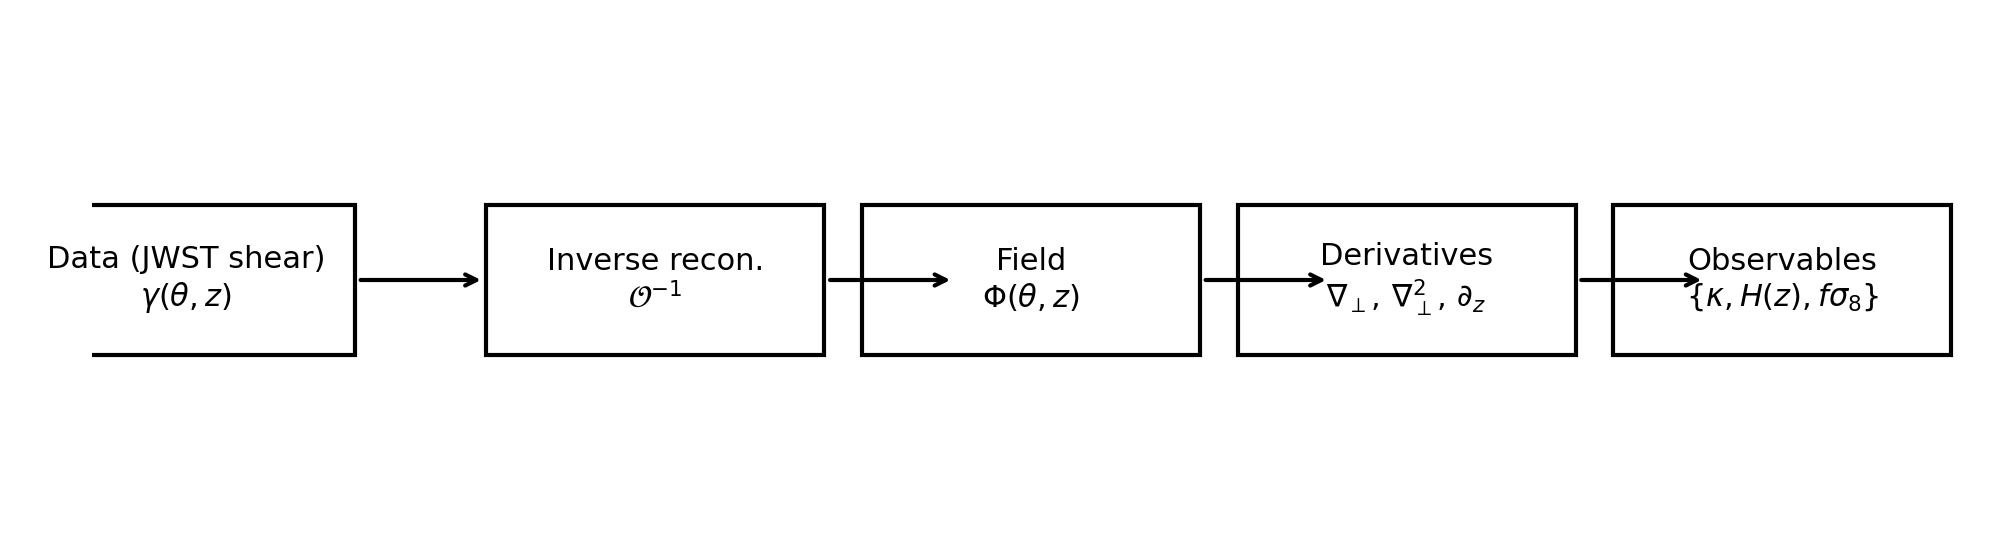
\includegraphics[width=\linewidth]{fig_pipeline.png}
\caption{Pipeline view: data $\rightarrow$ inverse reconstruction $\rightarrow$ inferred field $\Phi(\bm{\theta},z)$ $\rightarrow$ direct differential operators $\rightarrow$ observable set.}
\end{figure}

\begin{figure}[h!]
\centering
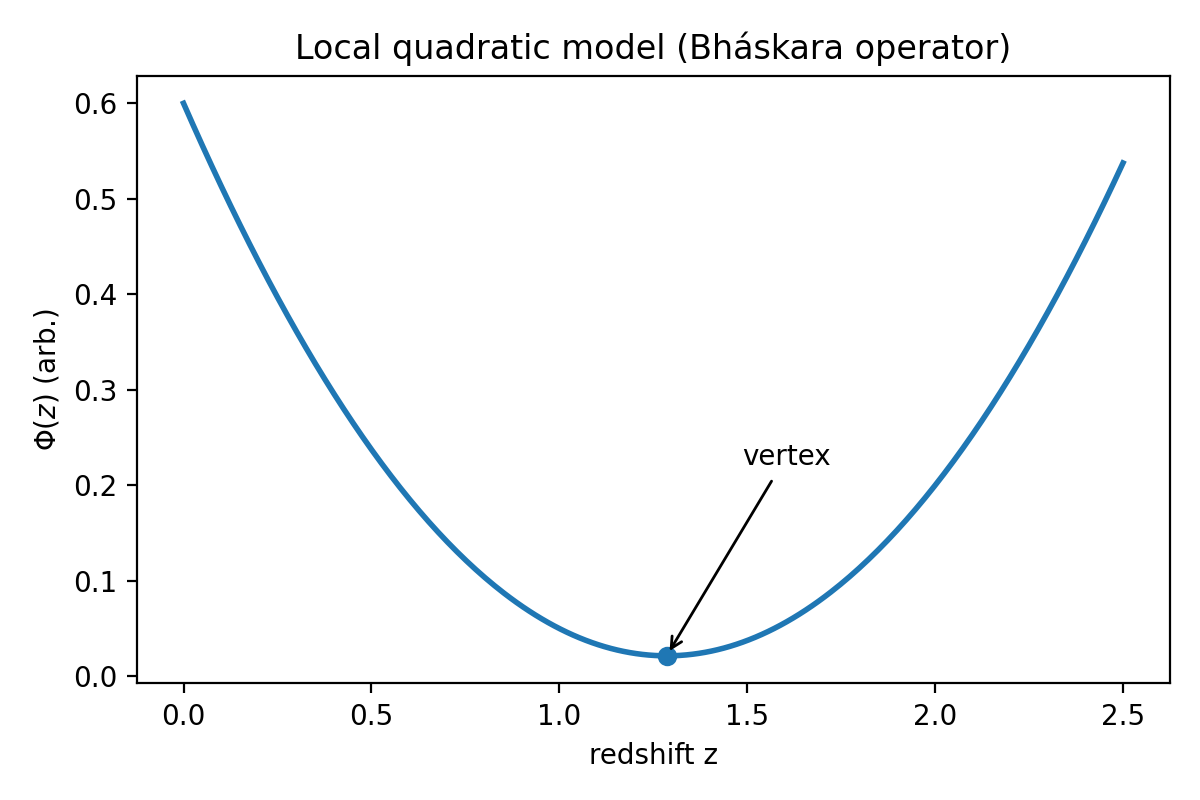
\includegraphics[width=0.78\linewidth]{fig_quadratic.png}
\caption{Local quadratic (Bh\'askara) model for the mean field $\Phi(z)$; the vertex indicates a stable/transition epoch.}
\end{figure}

\begin{figure}[h!]
\centering
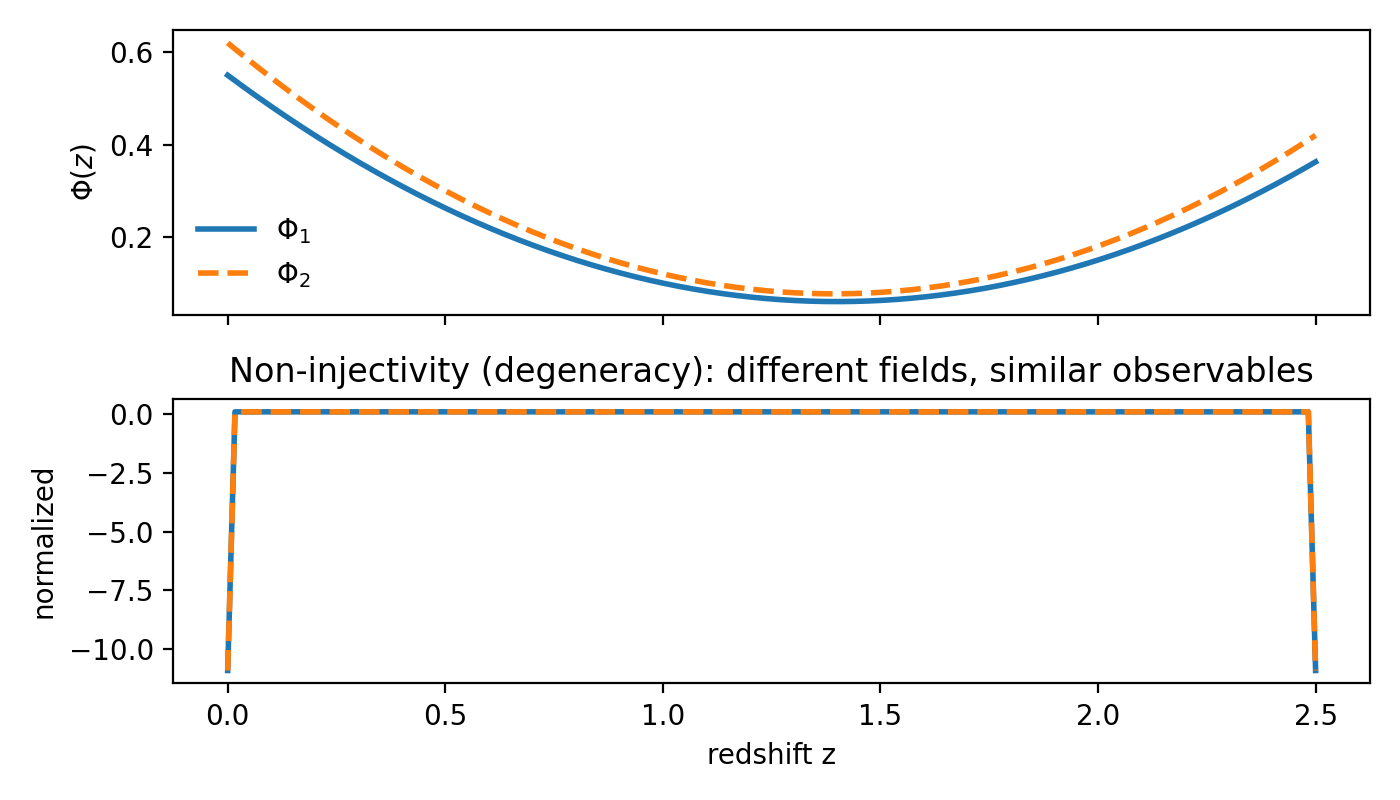
\includegraphics[width=0.90\linewidth]{fig_degeneracy.png}
\caption{Illustration of non-injectivity: distinct field trajectories can yield similar observable proxies, motivating priors/regularization and multi-probe anchoring.}
\end{figure}

\begin{figure}[h!]
\centering
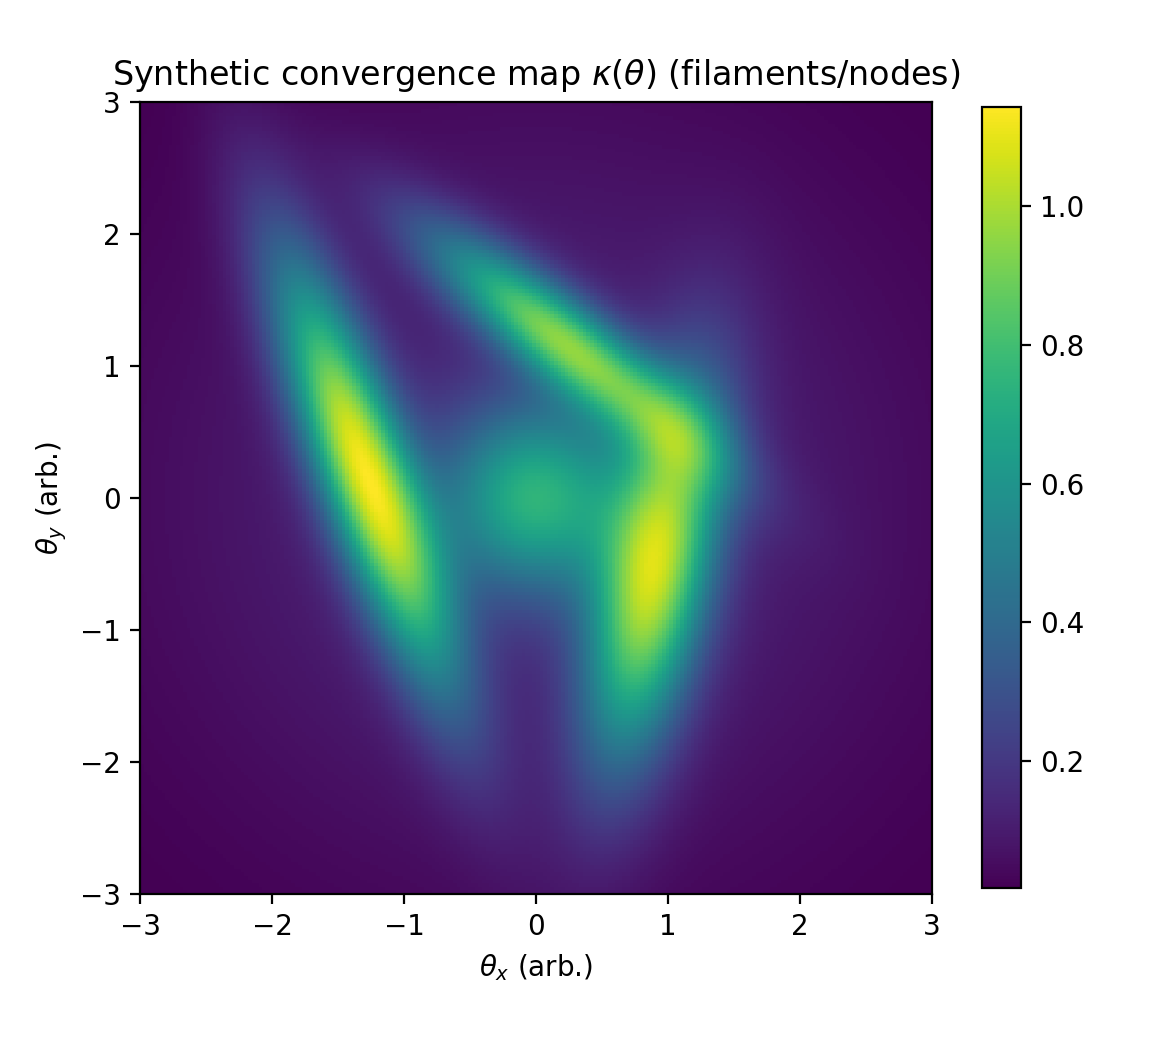
\includegraphics[width=0.70\linewidth]{fig_kappa_field.png}
\caption{Synthetic convergence map $\kappa(\bm{\theta})$ exhibiting filamentary ridges and nodes, representing the geometric targets of weak-lensing reconstruction.}
\end{figure}

\section{Conclusion}
The core result is a compact unification: observables are differential shadows of an inferred light-cone field, while reconstruction is necessarily regularized and degenerate. This reframes the ``dark sector'' as geometry plus inference: the map is not a photo, but a stable solution to an inverse problem constrained by multiple probes.

\end{document}
